\documentclass[10pt,a4paper]{article}
\usepackage{ucs}
\usepackage[utf8x]{inputenc}
\usepackage{amsmath}
\usepackage{amsfonts}
\usepackage{amssymb}
\usepackage[pdftex]{graphicx}

\usepackage[slovene]{babel}
\usepackage{lmodern}
\usepackage[T1]{fontenc}

\author{Vida Groznik, Anže Starič}
\title{Spomin}

\begin{document}
\maketitle
\newpage

\section{Uvod}
Spomin igra pomembno vlogo v našem življenju, saj predstavlja osnovo za učenje, sklepanje in razumevanje. Brez spomina bi dojemali le sedanjost in nebi mogli razumeti vzročnosti, saj bi do trenutka, ko bi videli rezultat neke akcije že pozabili, da smo akcijo izvedli.

Spomin v grobem delimo na eksplicitni (deklarativni) in implicitni (nedeklarativni) spomin. Kadar govorimo preprosto o spominu najpogosteje mislimo na {\bf eksplicitni spomin}. Do eksplicitnih spominov lahko dostopamo zavestno, enostavno jih tvorimo, ravno tako enostavno jih pozabljamo.

{\bf Implicitnega spomina} po drugi strani ne moremo uporabljati zavestno, vendar naučena opravila lahko opravljamo tudi brez zavestnega priklica (vožnja kolesa, prostoročno tipkanje, ...). Za tvorjenje implicitnih spominov potrebujemo več ponavljanja in vaje kot za tvorjenje eksplicitnih spominov, vendar jih zato težje pozabimo.

\section{Eksplicitni spomin}
Kot smo omenili v uvodu, eksplicitne spomine tvorimo in do njih dostopamo zavestno. Spominsko delovanje ločimo na pet procesov: {\it pozornost}, {\it vkodiranje}, {\it shranjevanje}, {\it konsolidacija} in {\it obnavljanje informacij}. {\it Pozornost} je sposobnost osredotočanja na določeno nalogo in igra pomembno vlogo pri izboru informacij, ki vstopajo v spominski proces. Drugi korak je {\it vkodiranje}, ki predstavlja registracijo informacij med procesom učenja. Če lahko informacijo povežemo z že znanimi asociacijami, je postopek vkodiranja bolj učinkovit. Ko je informacija vkodirana je {\it shranjena} v kratkoročni spomin. {\it Konsolidacija} je postopek organizacije kompleksnih informacij, pri katerem se prenesejo v dolgoročni spomin. Pri dostopanju do informacij gre za procese {\it obnavljanja informacij}, poznamo spontan priklic, priklic s pomočjo namiga in prepoznavanje. S priklicom in prepoznavanjem najlažje merimo sposobnost posameznikovega spominskega sistema.

Postopno pozabljanje je običajen proces našega spominskega sistema, kadar pa pride do večje izgube spomina, ki je posledica bolezni ali poškodbe govorimo o amneziji. Poznamo dve vrsti amnezije, {\it retrogradno amnezijo}, pri kateri gre za izgubo spominov pred poškodbo in {\it anterogradno amnezijo}, pri kateri gre za nezmožnost tvorjenja spominov po poškodbi.

\subsection{Hipokampus}
O pomembni vlogi hipokampusa pri tvorbi in hrambi deklarativnih spominov nam govori amnezija, ki nastane kot rezultat odstranitve obeh temporalnih režnjev. Posledice odstranitve si oglejmo na primeru bolnika H.M.

\subsubsection{Bolnik H.M.}
Pri bolniku H.M so se okrog desetega leta začeli pojavljati epileptični napadi. Z leti so postajali vse hujši, vključevali so tresenje, grizenje jezika in izgubo zavesti. Ker zaradi epilepsije kljub jemanju zdravil ni mogel normalno delati, so mu pri 27 letih med operacijo izrezali 8 cm medialnih delov obeh temporalnih režnjev, kar vključuje del korteksa, amygdalo in dve tretjini hippocampusa. Po operaciji so se epileptični napadi prenehali.

Odstranitev temporalnih režnjev ni vplivala na zavedanje, inteligenco ali osebnost bolnika H.M., vendar se je pri njem pojavila huda oblika amnezija. Amnezija je delno retrogradna, saj je izgubil spomin o dogodkih nekaj let pred operacijo, hujša pa je njena anterogradna oblika. Bolnik lahko prikliče nekatere dogodke iz otroštva, vendar pa se ne more spomniti nekoga, ki ga je videl pred nekaj minutami. Bolnik si ni zapomnil niti zdravnice, katero je skoraj 50 let videval vsak dan. Če na njem izvajamo poskus, pri katerem si mora bolnik zapomniti določeno število, nato pa njegovo pozornost preusmerimo drugam, bolnik ne le pozabi število, temveč pozabi tudi, da smo mu kadarkoli dali nalogo, da si število zapomni.

Bolnik ima ohranjen dolgoročni spomin, saj se spomni nekaterih dogodkov iz otroštva. Ravno tako je ohranjen delovni spomin, saj si lahko s ponavljanjem zapomni seznam števil, vendar takoj, ko pozornost preusmeri nekam drugam seznam števil pozabi. Na podlagi bolnika H.M. lahko sklepamo, da hipokampus igra pomembno vlogo pri tvorbi in hranjenju kratkotrajnega spomina.

\subsubsection{Vloga medialnega temporalnega režnja}
Poleg hippocampusa se na medialnem temporalnem režnju nahajata še rhinalni sulcus in parahippocampalni cortex. Medialni temporalni reženj informacije prejema iz asociacijskega področja, ki vsebuje močno obdelane informaciej iz vseh modalnosti. Vhod torej predstavljajo kompleksne predstavitve vhodov s čutil, pri katerih se lahko mešajo modalnosti. Glavna izhodna povezava je {\bf fornix}, ki potuje mimo talamusa in se konča v hipotalamusu.

\begin{figure}[h]
  \centering
    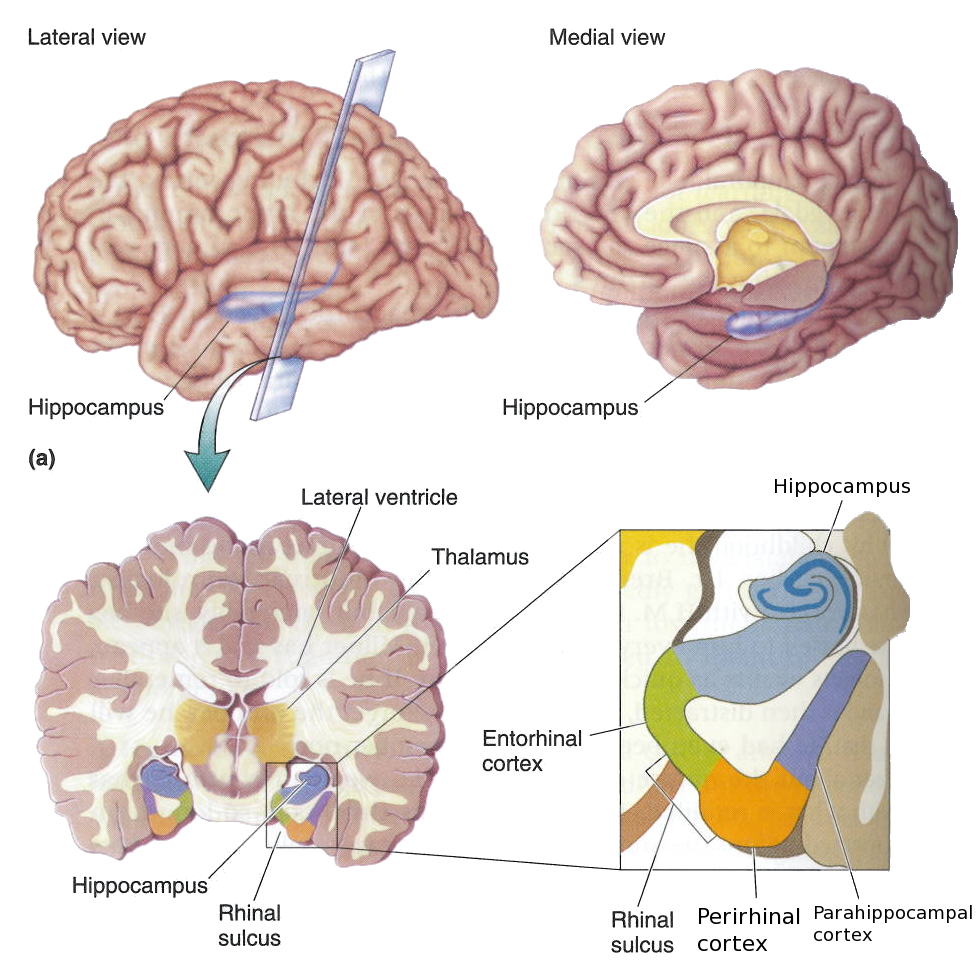
\includegraphics[width=1.0\textwidth]{LokacijaHippocampusa.png}
  \caption{Kje se nahaja hippocampus}
  \label{sHippocampus}
\end{figure}

\section{Implicitni spomin}
\subsection{Proceduralni spomin}
Za proceduralni spomin bi v grobem lahko rekli, da je to spomin za opravljanje različnih nalog. Ko se pojavi potreba po opravljanju neke naloge, se avtomatsko prikliče in uporabi proceduralni spomin, ki vsebuje tako kognitivne kot tudi motorične spretnosti. Proceduralni spomin je vrsta dolgoročnega spomina, natančneje implicitnega spomina.

\subsubsection{Anatomska struktura}
Striatum in bazalni gangliji\\
cerebellum\\
limbični sistem

\subsubsection{Fiziologija}
Dopamin\\
sinapsa

\subsubsection{Testi}

\subsubsection{Motnje}
Alzheimerjeva bolezen in demenca\\
Sindrom Gilles de la tourete\\
Virus HIV\\
Huntingtonova bolezen\\
Obsesivna kompulzivna motnja (OCD)\\
Parkinsonova bolezen\\
Šizofrenija

\subsubsection{Vpliv drog}
Alkohol\\
Kokain\\
Psihostimulanti

\section{}
\end{document}